\chapter{Lua程式碼}
\section{Robot控制}
\begin{figure}[hbt!]
\begin{center}
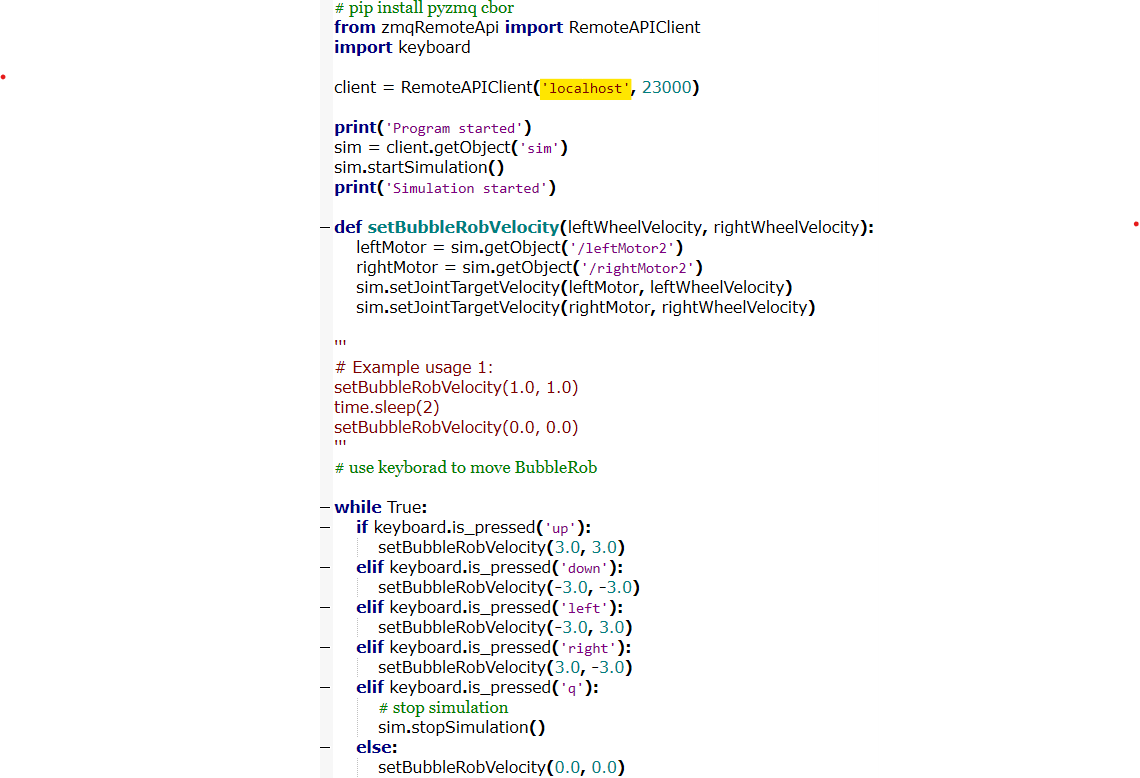
\includegraphics[width=16cm]{localhost_zmq}
\caption{\Large 本機操控}\label{localhost_zmq}
\end{center}
\end{figure}
以Lua程式在模擬環境中控制機器人運行。\\

\begin{figure}[hbt!]
\begin{center}
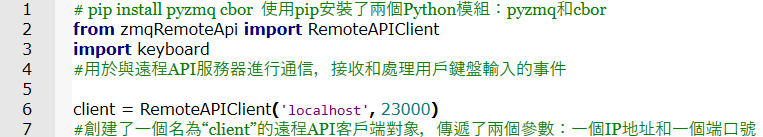
\includegraphics[width=16cm]{zmq-pip install}
\caption{\Large pip install}\label{zmq-pip install}
\end{center}
\end{figure}
(圖.\ref{zmq-pip install})使用 RemoteAPIClient 來連接遠端的 API 服務器,以及使用 keyboard 函式庫來控制鍵盤。\\
\newpage

\begin{figure}[hbt!]
\begin{center}
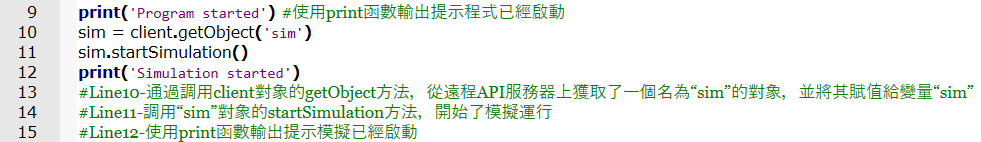
\includegraphics[width=16cm]{zmq-仿真環境}
\caption{\Large 仿真環境}\label{zmq-仿真環境}
\end{center}
\end{figure}
(圖.\ref{zmq-仿真環境})先使用 print 函式輸出一個提示訊息,表示程式已經啟動。接著,使用 RemoteAPIClient 物件的 getObject 方法來從遠端 API 服務器上獲取一個名為 sim 的物件。再呼叫 sim 物件的 startSimulation 方法來啟動模擬器的運行。最後,使用 print 函式輸出模擬器已經啟動。\\
\begin{figure}[hbt!]
\begin{center}
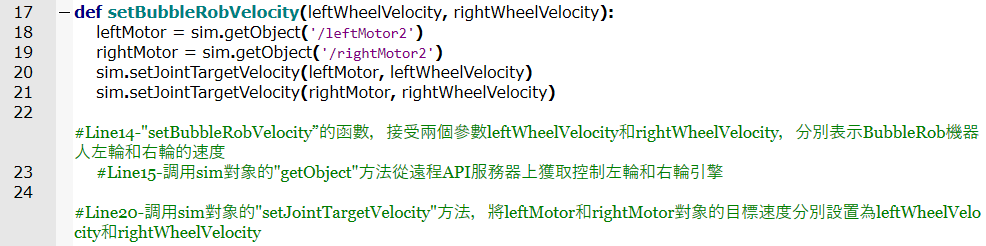
\includegraphics[width=16cm]{zmq-控制左右輪速度}
\caption{\Large 控制左右輪速度}\label{zmq-控制左右輪速度}
\end{center}
\end{figure}

(圖.\ref{zmq-控制左右輪速度})leftWheelVelocity 和 rightWheelVelocity,分別表示左輪和右輪的速度。sim.getObject 獲取 leftMotor2 和 rightMotor2馬達物件。sim.setJointTargetVelocity 方法來設定它們的目標速度。此段程式碼可以控制機器人的移動。\\
\newpage
\section{聯機控制}
\begin{figure}[hbt!]
\begin{center}
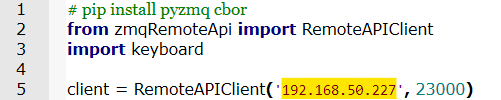
\includegraphics[width=16cm]{zmq-聯機}
\caption{\Large 聯機參數}\label{zmq-聯機}
\end{center}
\end{figure}
(圖.\ref{zmq-聯機})指定了一個 IP 位址 192.168.50.227 和一個端口號 23000 作為連接遠端 API 服務器的方式。RemoteAPIClient 可以從遠端 API 服務器獲取數據或控制遠端機器人的運動。\\
\newpage
\section{記分板}
\begin{figure}[hbt!]
\begin{center}
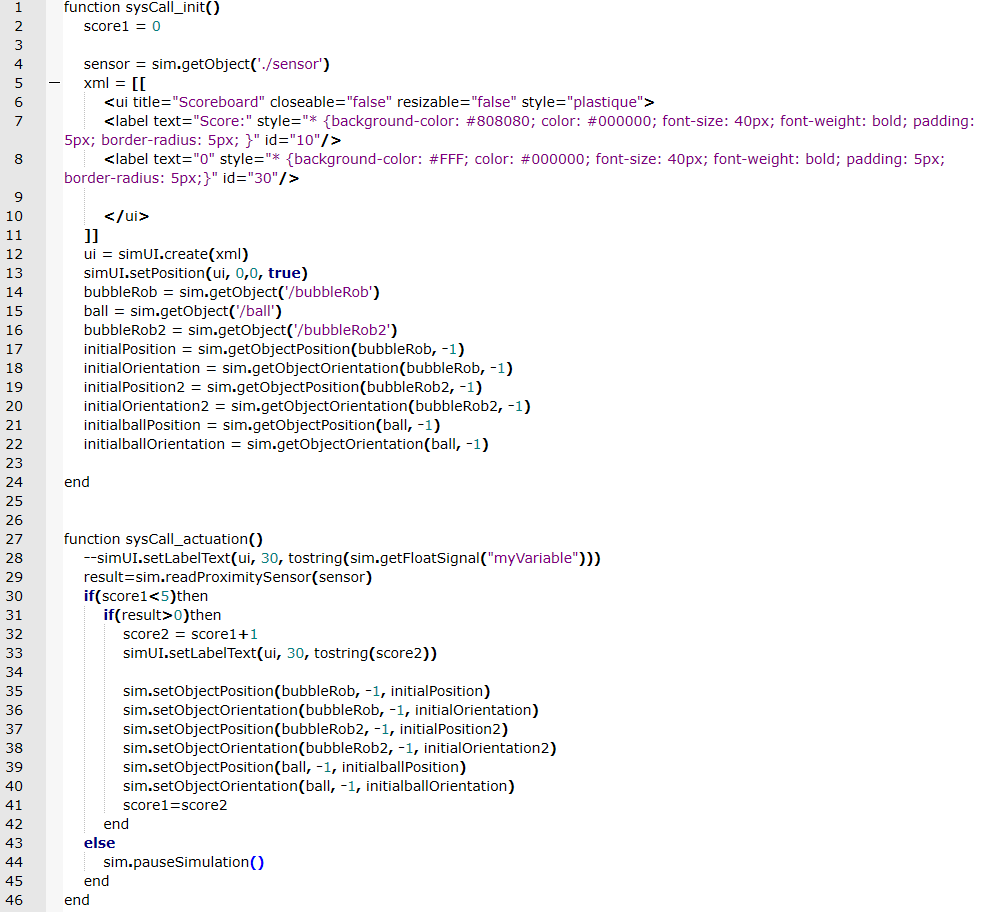
\includegraphics[width=16cm]{Scoreboard}
\caption{\Large 記分板}\label{Scoreboard}
\end{center}
\end{figure}
透過 Lua 程式建立記分板,設計樣式,給予偵測定義。\\
\newpage
\begin{figure}[hbt!]
\begin{center}
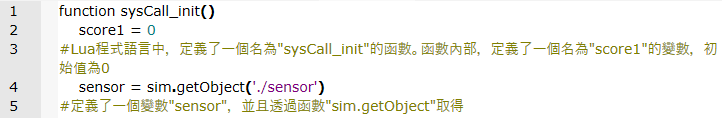
\includegraphics[width=16cm]{sc-senor}
\caption{\Large sensor}\label{sc-senor}
\end{center}
\end{figure}

(圖.\ref{sc-senor})sysCall init 的函式建立了一個名為 score1 的變數,並將它的值設定為 0使用 sim.getObject 方法來獲取一個名為 sensor 的物件,並將它儲存在 sensor 變數中。\\
\begin{figure}[hbt!]
\begin{center}
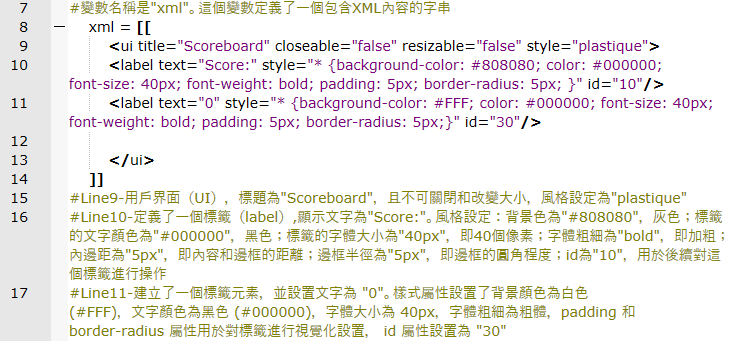
\includegraphics[width=16cm]{sc-xml}
\caption{\Large xml}\label{sc-xml}
\end{center}
\end{figure}

(圖.\ref{sc-xml}存儲在名為 xml 的變數中的 XML 代碼,它描述了一個顯示得分的視窗界面。ui 標籤中,有兩個 label 標籤,分別用來顯示 "Score:" 和得分。\\
\begin{figure}[hbt!]
\begin{center}
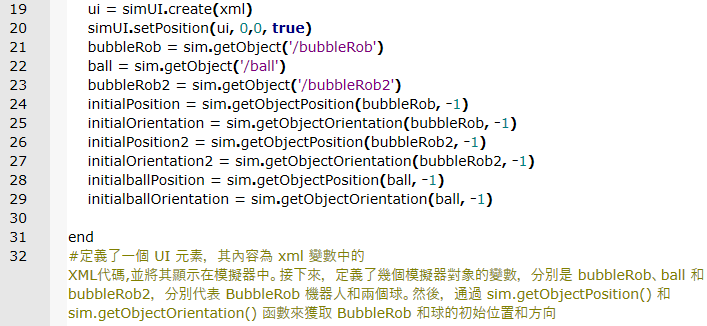
\includegraphics[width=16cm]{sc-ui}
\caption{\Large ui}\label{sc-ui}
\end{center}
\end{figure}

\newpage
(圖.\ref{sc-ui}建立使用者介面 (ui),然後設定該介面的位置為 (0, 0)。sim.getObject 函式從仿真場景中取得了三個物體,sim.getObjectPosition 和 sim.getObjectOrientation 函式取得了這些物體的初始位置和初始方向,這段程式碼是用來建立仿真場景中物體的初始位置和初始方向。\\
\begin{figure}[hbt!]
\begin{center}
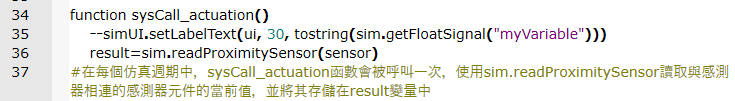
\includegraphics[width=16cm]{sc-syscall}
\caption{\Large syscall}\label{sc-syscall}
\end{center}
\end{figure}

(圖.\ref{sc-syscall}sysCall-actuation的函式使用 sim.readProximitySensor 函式讀取一個接近傳感器的數據,並將結果儲存在 result 變數中。\\
\newpage
\begin{figure}[hbt!]
\begin{center}
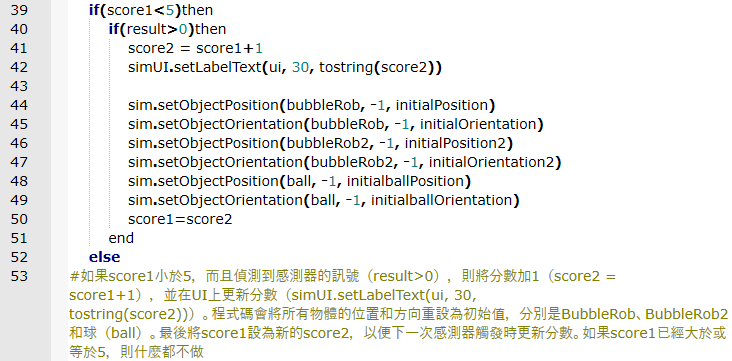
\includegraphics[width=16cm]{sc-if-else}
\caption{\Large if-else}\label{sc-if-else}
\end{center}
\end{figure}

(圖.\ref{sc-if-else}這段程式碼的主要作用是檢查分數是否小於5分,如果 score1 的值小於5,且 result 大於0,則將分數加1並在UI上更新分數。如果 score1 的值已經達到或超過了5分,則會跳過。\\
\begin{figure}[hbt!]
\begin{center}
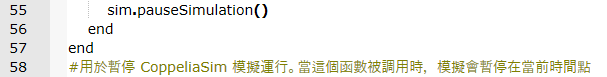
\includegraphics[width=16cm]{sc-pause}
\caption{\Large pause}\label{sc-pause}
\end{center}
\end{figure}

(圖.\ref{sc-pause}檢查分數是否小於5分。如果分數達到5分或更高,它會暫停仿真並結束程式執行。\\













